%!TEX root = ../../Master.tex
\subsection{Directed and Undirected Graphs}

\Cref{fig:labeled_Directed_undirected} shows two graphs, one is directed and the other is undirected. Graph 1 is undirected and does not have a specific direction. Graph 2 is directed which means the edges is one way only. The arrows indicates the direction the edges allow. This means vertex 1 can go to vertex 2 and 3, but neither can go back. 


\begin{figure}[ht!]
    \centering
    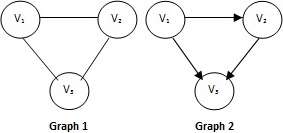
\includegraphics[width=0.5\textwidth]{Directed_undirected.png}
    
    \caption{Graph 1 is directed and graph 2 is undirected. From \cite{dir_pic}}\label{fig:labeled_Directed_undirected}


  \end{figure}